\newpage
\section{DESARROLLO Y ANÁLISIS DE RESULTADOS}
A continuación se muestran los métodos de desarrollo utilizados para resolver cada uno de los problemas planteados, así como la funciones utilizadas, el \textit{hardware} construido y los resultados obtenidos:

\subsection{Desarrollo de la solución}
En esta sección, se explica el proceso de desarrollo de \textit{hardware} y \textit{software} utilizado para diseñar e implementar la solución planteada para el proyecto: 

%-----Harware-------
% Dispensador de comida/Servo/Stepper
\subsubsection{Dispensador de comida/Servo/Stepper}
Inicialmente se realizó una búsqueda de posibles diseños existentes para tomar ideas y construir el dispensador de comida.

\begin{figure}[H]
\centering
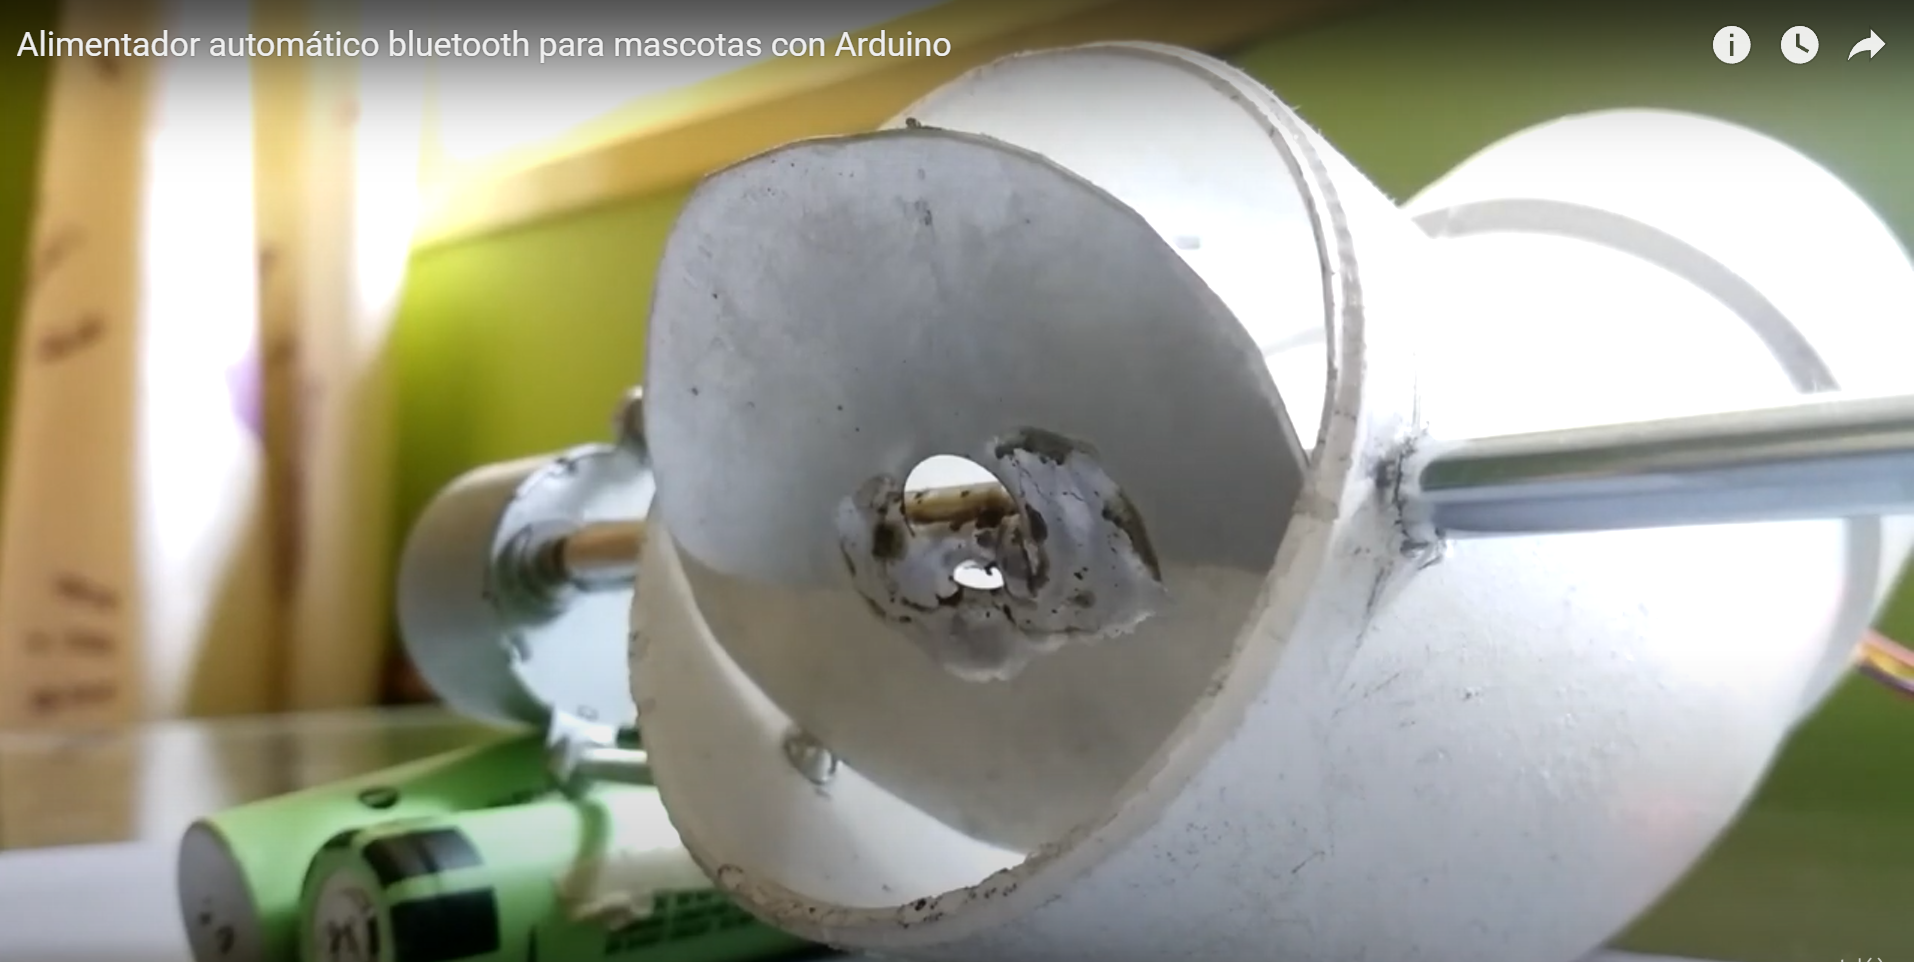
\includegraphics[width=90mm]{./Figuras/Desarrollo_Analisis/Diseño1}
\caption{Primer diseño consultado. (Fuente: \cite{TD_2019})}
\label{fig:DC}
\end{figure}

Este primer diseño es muy interesante, note que hace uso de un stepper motor así como de una especia de varille que controla la tapa de apertura del contenedor. Inicialmente se implementó uno diseño prácticamente idéntico, sin embargo un aspecto importante a considerar era que en el escenario de este proyecto, se desea que el reservorio principal tenga alimento para más de un refill. Esto generaba que la cantidad e alimento fuera considerable y que su peso cayera sobre la integridad de la tapa. Por que la tapa al intentar abrir, necesitaba el torque necesario para levantar el alimento. Al seguir consultando diseños propuestos, se encontró el siguiente:

\begin{figure}[H]
\centering
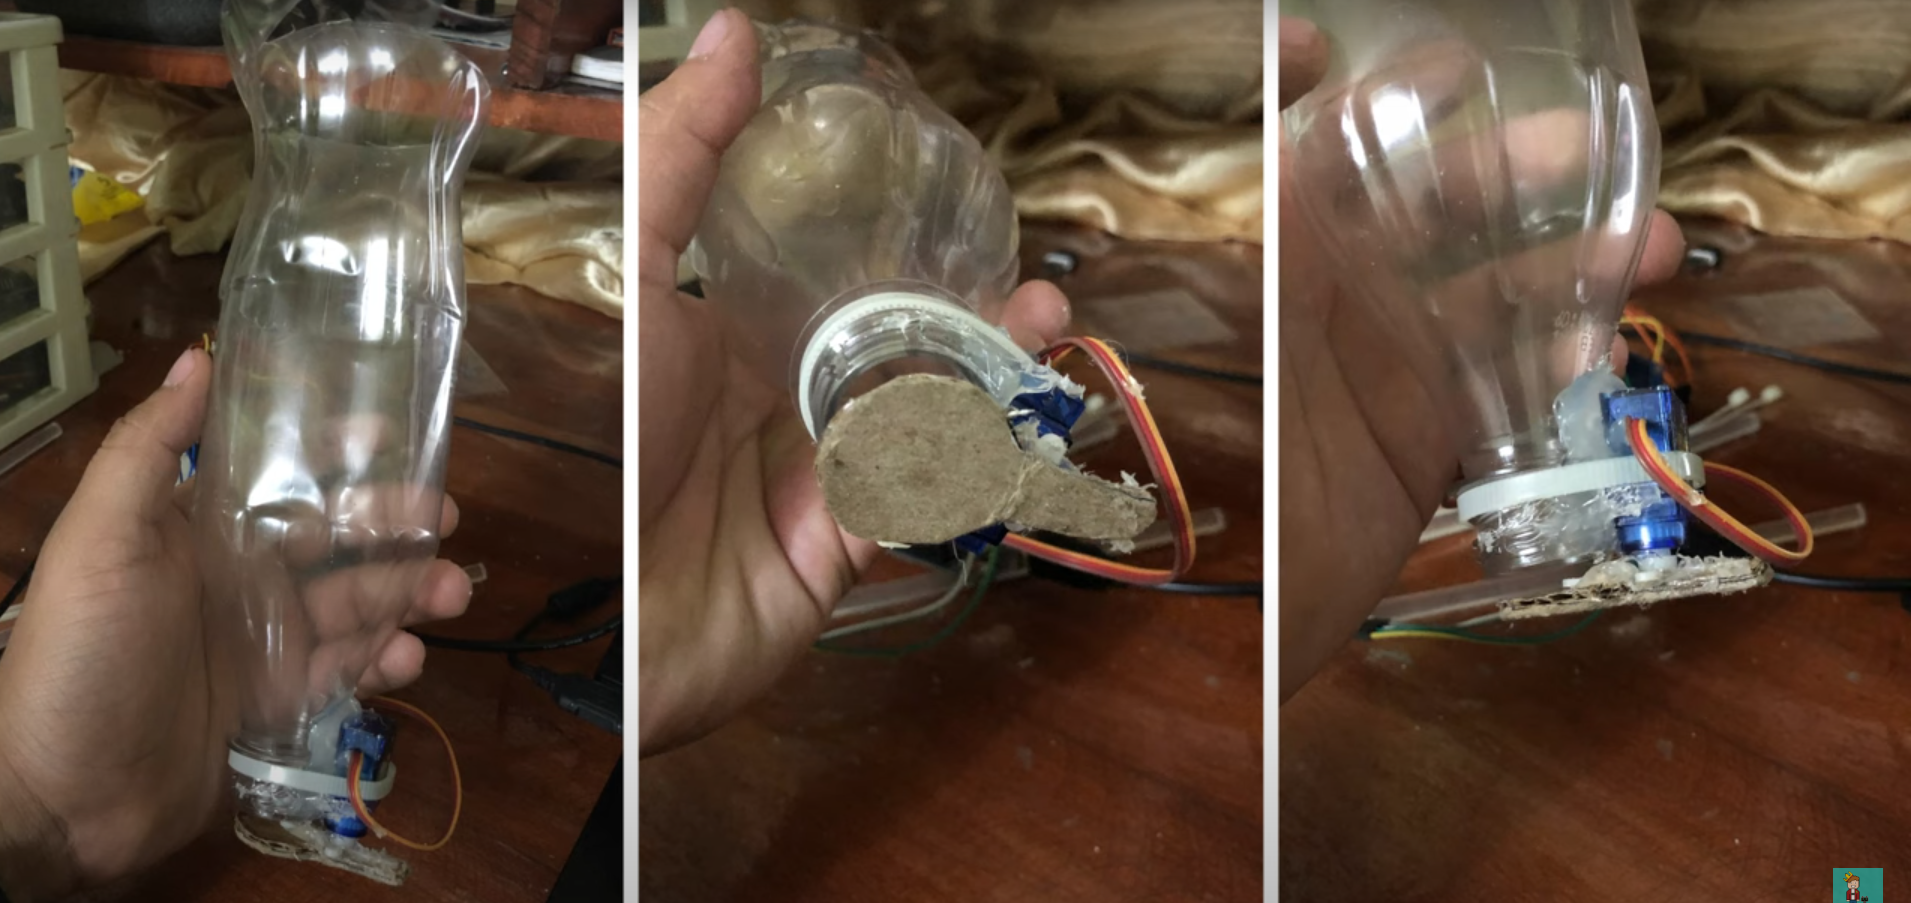
\includegraphics[width=90mm]{./Figuras/Desarrollo_Analisis/Diseño2}
\caption{Segundo diseño consultado. (Fuente: \cite{SalvaTronic_2024})}
\label{fig:DC2}
\end{figure}
De este diseño lo que resultó llamativo fué el uso del servomotor. Por lo qué de aca surgió la idea de migrar al uso de servo y crear una especia de portón corredizo que permitiera el flujo de comida. Para este portón se utilizó una malla reciclada, que normalmente se encuentra en la base de los sartenes de cocina. El diseño propuesto de dispensador de alimento para este trabajo el siguiente:

\begin{figure}[H]
\centering
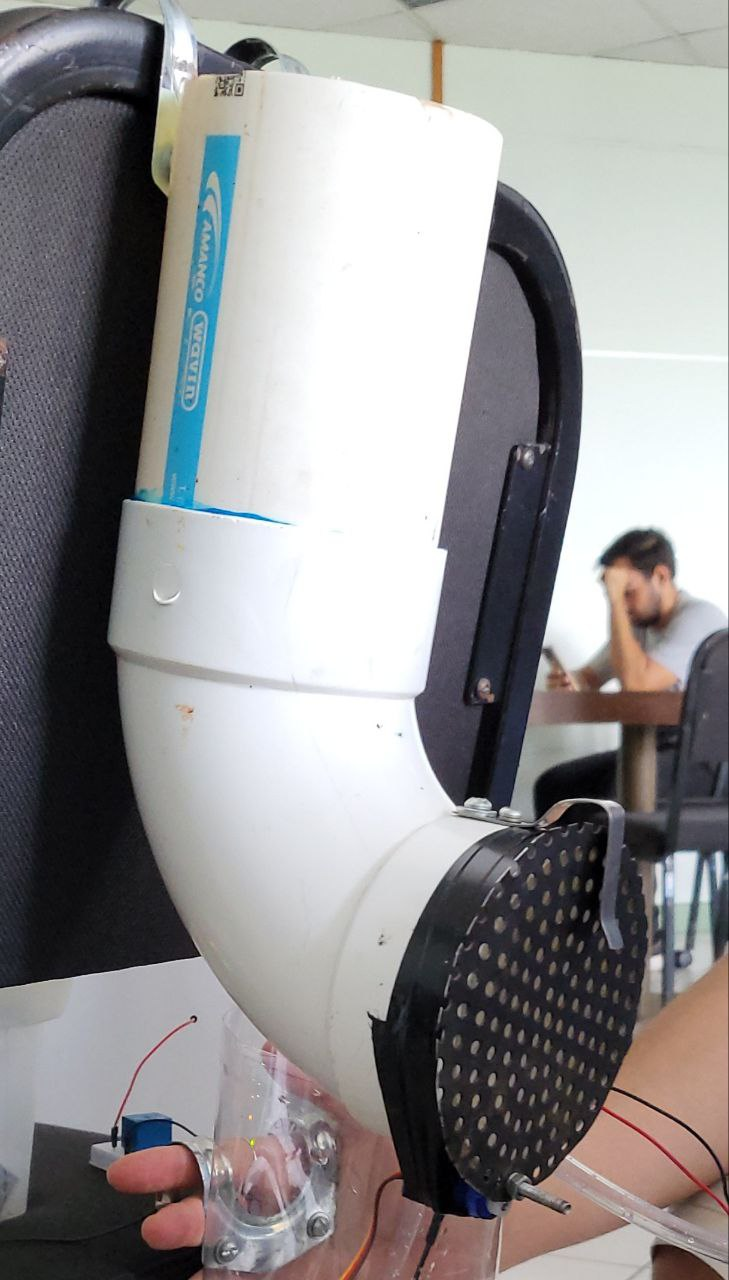
\includegraphics[scale=0.3]{./Figuras/Desarrollo_Analisis/diseño_final_dispensador_comida}
\caption{Diseño propuesto.}
\label{fig:DC3}
\end{figure}
Note que el diseño propuesto es una combinación de las ideas consultadas, más mejoras como por ejemplo el aumento de capacidad de almacenamiento pegando más tubo al codo. Se añadió una placa metálica plateada de seguridad, que mantiene la tapa del reservorio presionada, evitando así cualquier desperdicio o fuga de alimento. Note que se esta usando el servomotor, es importante mencionar que inicialmente se realizaron pruebas de funcionamiento usando Arduino con sus pines de 5V. Sin embargo una vez se consiguió el microcontrolador ESP8266 que es el microcontrolador seleccionado para este proyecto, este solo cuenta con pines 3.3v y menos corriente. Por lo que se percibió una disminución en el rendimiento y velocidad de operación del servomotor.


% Dispensador de agua/Bomba/Rele/Transistor
\subsubsection{Dispensador de agua/Bomba/Relé/Transistor}
Para lo que es el reservorio de agua, se decidió utilizar una botella plástica esto por disponibilidad del material, su naturaleza resistente a los líquidos y su capacidad de almacenaje. En ambos reservorios tanto de comida como de agua, se añadió un soporte, que permite apoyar los reservorios a cualquier tipo de silla o mueble.

\begin{figure}[H]
\centering
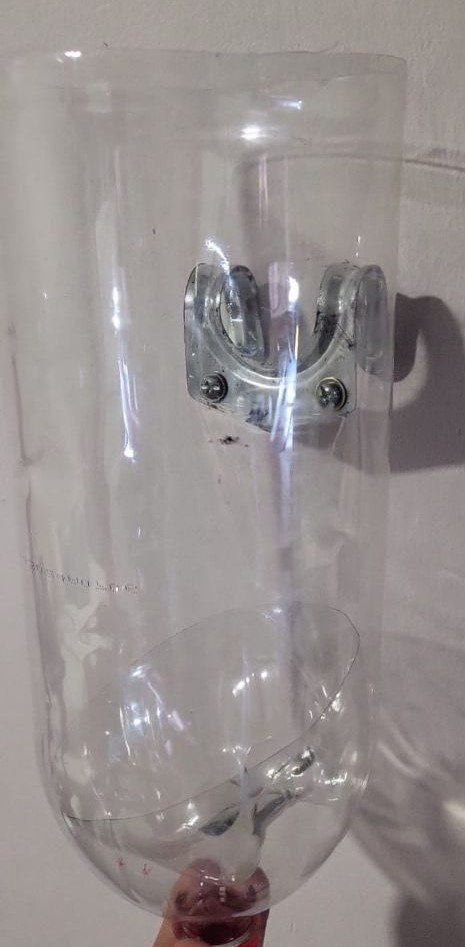
\includegraphics[scale=0.3]{./Figuras/Desarrollo_Analisis/reservorio_agua}
\caption{Imagen del Reservorio de agua con soporte.}
\label{fig:botella}
\end{figure}

Se obtuvo una bomba de agua del tipo sumergible, que no cuenta con alguna patilla de control. Por lo que se vió la necesidad de proponer un circuito de control con relé. Inicialmente antes de tener el ESP8266, se realizaron simulaciones y pruebas con el pin de alimentación de arduino UNO de 3.3 V, en el que se lograba activar el relé. Sin embargo al momento de migrar al ESP8266, el relé no ese activaba a pesar de tener la misma tensión. En este momento al consultar la literatura nos damos cuenta que los pines GPIO del ESP8266 tienen una corriente de salida de hasta 12 mA, mientras que los de Arduino de hasta 40 mA en este momento se percibe que es un problema por baja corriente. Investigando se encontró el circuito propuesto en \cite{Sergio_2020}, el cual resuelve este problema: 

\begin{figure}[H]
\centering
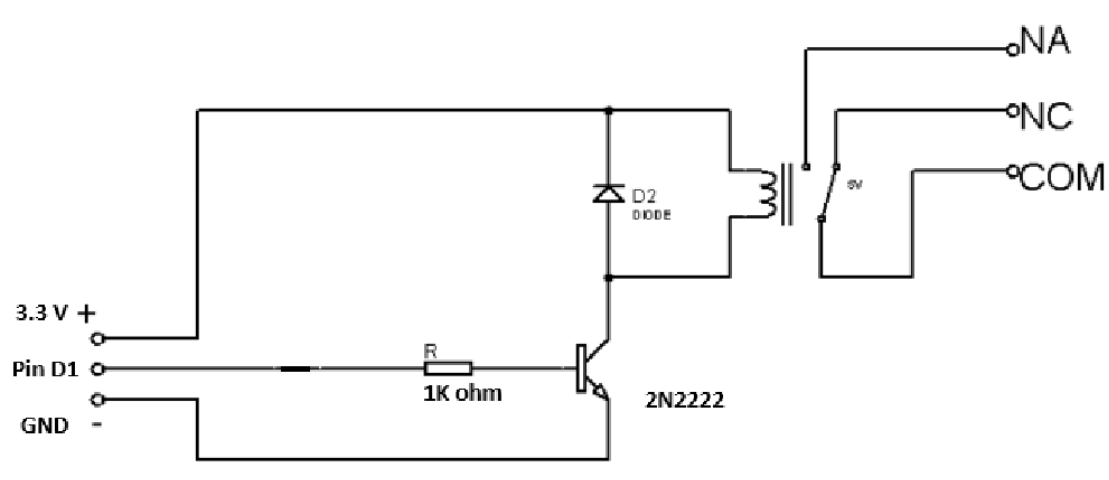
\includegraphics[scale=0.5]{./Figuras/Desarrollo_Analisis/Circuito_rele}
\caption{Imagen del Reservorio de agua con soporte.}
\label{fig:botella2}
\end{figure}

El uso de un transistor 2N2222 permite tener control sobre el relé usando una patilla GPIO del ESP8266 en la base del transistor. Así como elevar la corriente debido a la ganancia que poseen los transistores. El diodo se utiliza como protección a los picos generados en las transiciones del relé. De esta manera se logró realizar el control de la bomba con ESP8266.
\\
Un problema interesante que surgió en el bombeo entre el reservorio principal y la taza de agua del animal fué un fenómeno denominado como sifón. Un sifón es una diferencia de presión que permite que el agua fluya de un nivel más alto a uno más bajo, incluso sin la ayuda de la bomba.\cite{palomino2017analisis} Este fenomeno hacia que el agua fluyera hacia la taza del animal aun cuando la bomba se apagaba. La solución planteada fué variar la altura del reservorio principal.


\subsubsection{Tazas de agua y comida/Sensores ultrasónicos}
Para realizar las mediciones de distancia en las tazas de comida y agua, fue necesario colocar los sensores ultrasónicos en la parte superior de estas. Para fijar el sensor y evitar movimientos verticales y horizontales que insertaran ruido a las mediciones de nivel, se utilizó porcelana fría, la cual representa un buen material en la medida en que seca bastante rápido y evita cualquier movimiento. En la Figura \ref{fig:TS}, puede verse la forma en la que los sensores fueron colocados en cada taza:

\begin{figure}[H]
\centering
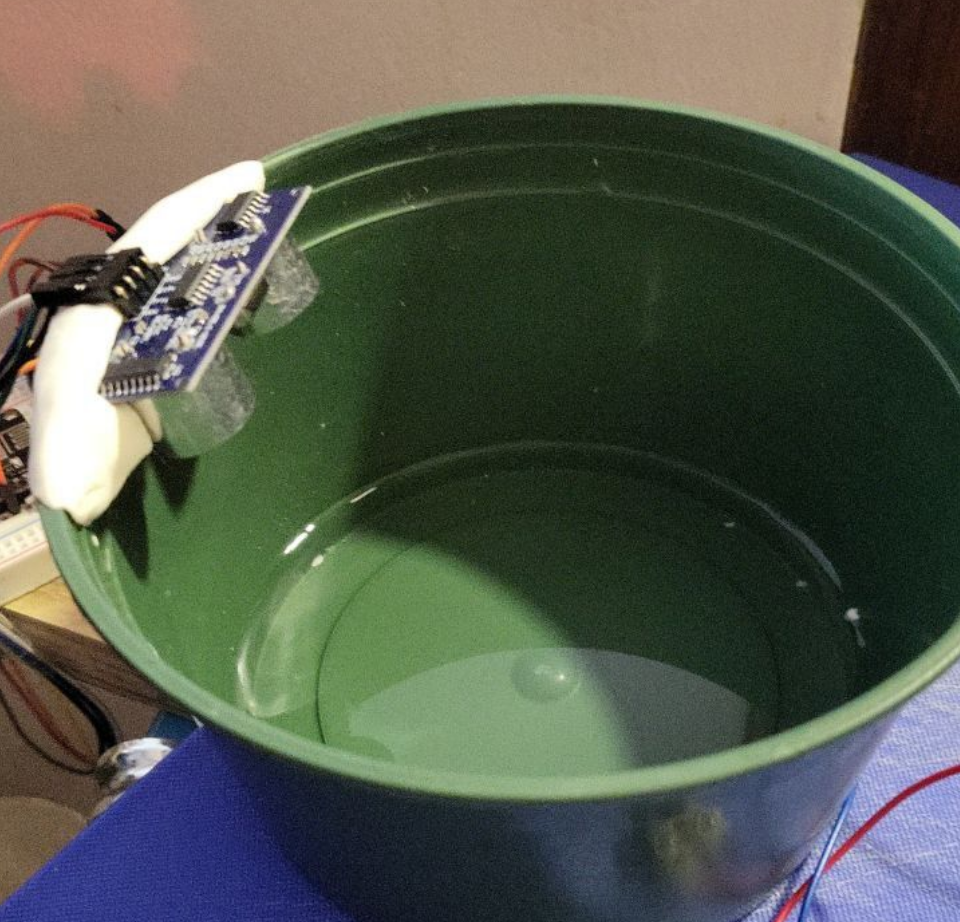
\includegraphics[width=90mm]{./Figuras/Desarrollo_Analisis/TS}
\caption{Taza de agua con el sensor ultrasónico adherido a este utilizando porcelana fría.}
\label{fig:TS}
\end{figure}

\subsubsection{Circuito general}
Una vez que se tenían todas las partes completadas, solamente restaba unir todas estas utilizando el microcontrolador elegido para el proyecto. En la Figura \ref{fig:CG} puede consultarse de manera general y a alto nivel el circuito construido:  

\begin{figure}[H]
\centering
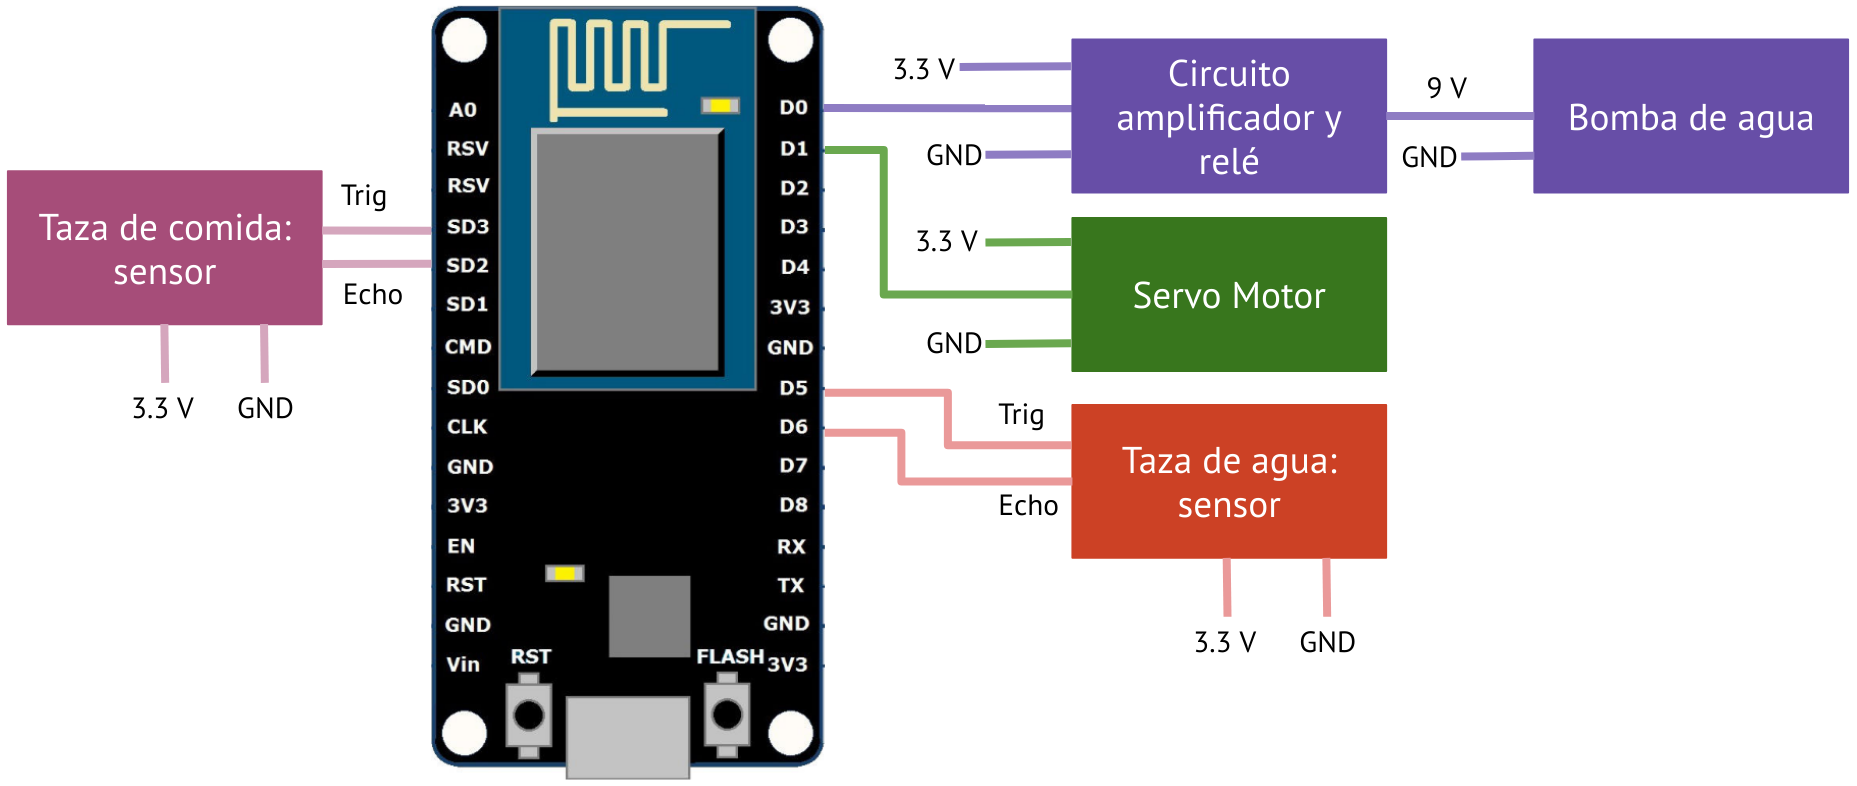
\includegraphics[width=155mm]{./Figuras/Desarrollo_Analisis/CG}
\caption{Disposición general del circuito utilizado para el proyecto. (Elaboración propia).} 
\label{fig:CG}
\end{figure}

Como puede verse en la Figura \ref{fig:CG}, el circuito está dividido en tres etapas: 
\begin{enumerate}
    \item \textbf{Tazas de agua y de comida}: cada un cuenta con un sensor ultrasónico que se encarga de la medición de proximidad del alimento y agua, resultando en un monitoreo constante del nivel en ambos casos. 

    \item \textbf{Servo motor}: este motor es controlador por el ESP8266, permite la distribución de comida en la taza de comida, cuando sea necesario. El motor tiene el objetivo de abrir el portón del contenedor principal de comida. 

    \item \textbf{Bomba de agua}: esta sección cuenta con dos partes. En primer lugar se tiene el circuito amplificador de corriente para poder accionar el relé de activación de la bomba de agua, este es alimentado por el ESP8266. En segundo lugar, se tiene la bomba de agua como tal, la cual se encargar de la distribución de agua desde el contender principal a la taza de agua cuando sea necesario. 
\end{enumerate}
A continuación se muestra el circuito completo conectado en su etapa de pruebas:
\begin{figure}[H]
\centering
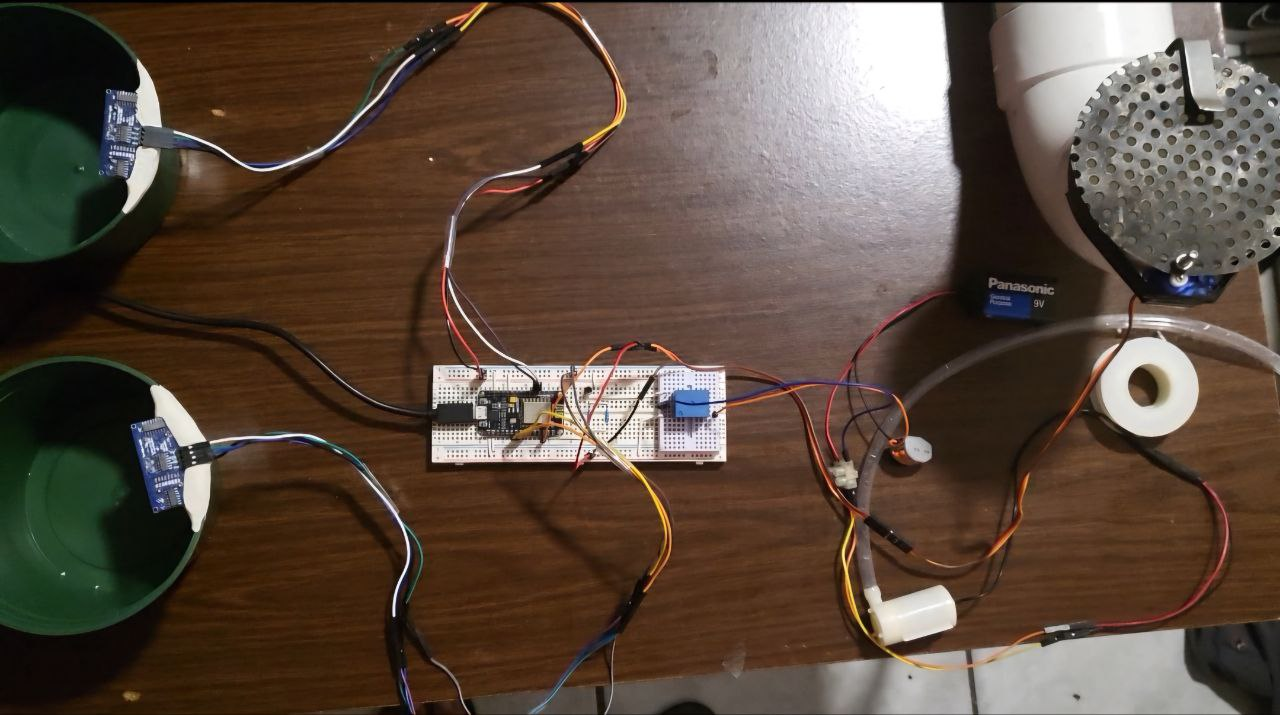
\includegraphics[width=155mm]{./Figuras/Desarrollo_Analisis/CG2}
\caption{Imagen del circuito completo en su etapa de pruebas. (Elaboración propia).} 
\label{fig:CG2}
\end{figure}

%-----Software------
\subsubsection{Desarrollo de \textit{software}}
A continuación podrá consultarse una descripción de alto nivel de cada una de las funciones implementadas en el código .ino:

\begin{itemize}
    \item \textbf{\texttt{setup()}}: esta corresponde a la función principal de configuración, en esta se configuran las siguientes partes: 
    \begin{itemize}
        \item \textbf{\texttt{setup\_servo()}}: se encarga de la configuración básica del servo motor. 
        \item \textbf{\texttt{setup\_pump()}}: se encarga de la configuración básica de los pines de control utilizados para controlar el circuito de amplificación que a su vez se encarga de controlar la bomba de agua.  
        \item \textbf{\texttt{setup\_ultrasonic()}}: configura los pines de de \textit{trigger} y \textit{echo} de los dos sensores ultrasónicos utilizados.  
    \end{itemize}

    \item \textbf{\texttt{distance\_measure(int trigPin, int echoPin)}}: esta función envía un pulso de 10 microsegundos al pin de disparo del sensor ultrasónico (trigPin), y luego mide el tiempo que tarda en recibir el pulso reflejado en el pin de eco (echoPin). Utiliza esta duración para calcular y retornar la distancia en centímetros.

    \item \textbf{\texttt{water\_level\_bowl(int trigPin, int echoPin)}}: mide la distancia desde el sensor ultrasónico ubicado en la taza de agua. Si la distancia medida es mayor o igual a 7 cm, se considera que la taza está vacía y se muestra un mensaje en el serial. Si se recibe una señal de Blynk para llenar la taza, la bomba de agua se activa hasta que la distancia medida sea menor a 4 cm. Durante este proceso, se envían los valores de nivel de agua a la aplicación Blynk.

    \item \textbf{\texttt{food\_level\_bowl(int trigPin, int echoPin)}}: mide la distancia desde el sensor ultrasónico ubicado en la taza de comida. Si la distancia medida es mayor o igual a 7 cm, se considera que la taza está vacía y se muestra un mensaje en el serial. Si se recibe una señal de Blynk para llenar la taza, el servo motor se mueve a 180 grados para dispensar comida hasta que la distancia medida sea menor a 5.5 cm. Durante este proceso, se envían los valores de nivel de comida a la aplicación Blynk.

    \item \textbf{\texttt{status\_checker()}}: verifica los niveles en las tazas de comida y agua. 

    \item \textbf{\texttt{loop()}}: Mantiene la conexión con el servidor de Blynk mediante \texttt{Blynk.run()}, gestionando la comunicación con la aplicación móvil. Además, llama a \texttt{status\_checker()} para monitorear y controlar los niveles de comida y agua en los recipientes y contenedores, tomando acciones en consecuencia.
\end{itemize}

\subsubsection{Arduino Cloud/Blynk}
Tal como había sido planteado al inicio del proyecto, se quería utilizar la plataforma Arduino Cloud para manejar el sistema construido utilizando IoT. A pesar de que se configuró e intentó la implementación de esta, se presentaron varios problemas:

\begin{itemize}
    \item Errores al intentar conectar el ESP8266 a la plataforma. A pesar de que el agente necesario fue instalado, la plataforma no era capaz de identificar el dispositivo todo el tiempo, lo que causaba inestabilidad al momento de hacer \textit{upload}.

    \item En las ocasiones en las que el dispositivo sí pudo conectarse a la plataforma, se tuvieron problemas con la conexión WiFi. El error correspondía a un problema con el \textit{broker} de  MqTT, ya que no podía acceder al puerto dispuesto para la comunicación, independientemente de la red en la que el dispositivo se conectara. 
\end{itemize}

Es por lo anterior que se decidió utilizar cambiar de plataforma y utilizar Blynk para realizar las mismas tareas planteadas para Arduino Cloud. La conexión entre la plataforma Blynk y el ESP8266 se logra mediante la función \texttt{Blynk.begin(auth, ssid, pass)}, que establece la conexión con el servidor de Blynk utilizando credenciales definidas. Dentro del bucle principal \texttt{loop()}, se llama continuamente a \texttt{Blynk.run()} para mantener activa la conexión y permitir la comunicación bidireccional. Los comandos y datos se intercambian a través de funciones como \texttt{BLYNK\_WRITE(V0)} y \texttt{BLYNK\_WRITE(V1)}, que responden a los cambios en los widgets de la aplicación, permitiendo controlar remotamente el nivel de comida y agua en las tazas.

\subsection{Análisis de los resultados}

% CASO A foto tazas vacías X / Impresion de terminal X / Foto de Dashboard X
\subsection{Caso A: Tazas Vacías}
A continuación se analiza el escenario en el que ambas tazas se encuentran vacías.

\begin{figure}[H]
\centering
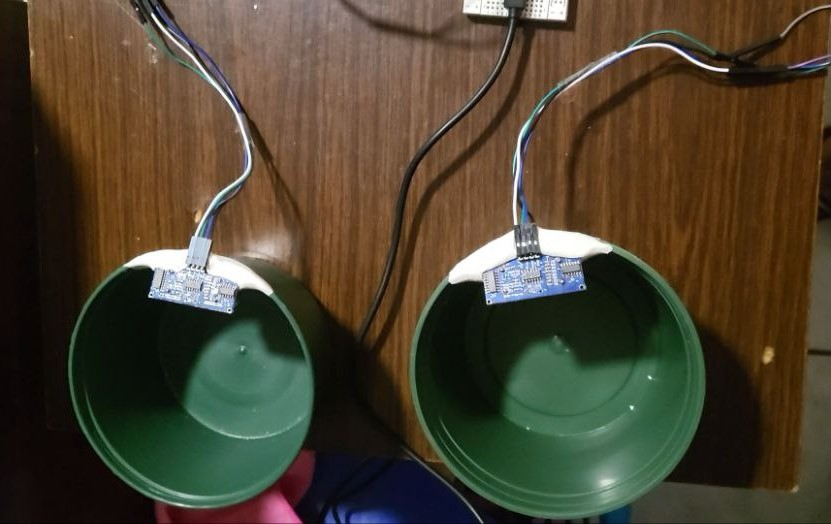
\includegraphics[width=110mm]{./Figuras/Desarrollo_Analisis/tazas_vacias}
\caption{Imagen del dispensador con las tazas vacías.} 
\label{fig:analisis1}
\end{figure}

En este escenario se espera que en terminal se realice la impresión que indique que tanto la taza de agua como la de comida se encuentran vacías. A continuación se muestra como efectivamente se cumple lo anterior:

\begin{figure}[H]
\centering
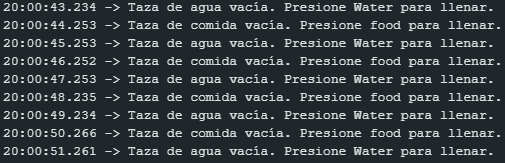
\includegraphics[width=100mm]{./Figuras/Desarrollo_Analisis/vacios}
\caption{Impresión en Serial monitor con las tazas vacías.} 
\label{fig:analisis2}
\end{figure}

Además se obtiene en el \textit{dashboard} de Blynk, que los niveles de las tazas reflejen valores bajos de acuerdo a su condición de vacíos:

\begin{figure}[H]
\centering
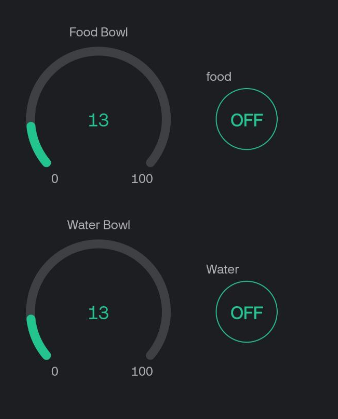
\includegraphics[width=80mm]{./Figuras/Desarrollo_Analisis/dash_vacios}
\caption{\textit{Dashboard} de Blynk con las tazas vacías.} 
\label{fig:analisis3}
\end{figure}

De este escenario A se puede analizar que se están imprimiendo lecturas de vacío esperadas. Esto indica que los sensores ultrasónicos están detectando adecuadamente cuando las tazas están vacías. El \textit{dashboard} muestra valores que concuerdan con lo que esta pasando en las tazas, por lo que la comunicación entre los sensores y el \textit{dashboard} funciona como se espera.

% CASO B llenando taza Agua X / Impresión en terminal X/ Foto del Dashboard X
\subsection{Caso B: Llenando taza Agua}
A continuación se analiza el escenario en el se acciona el botón de llenar taza de agua.

\begin{figure}[H]
\centering
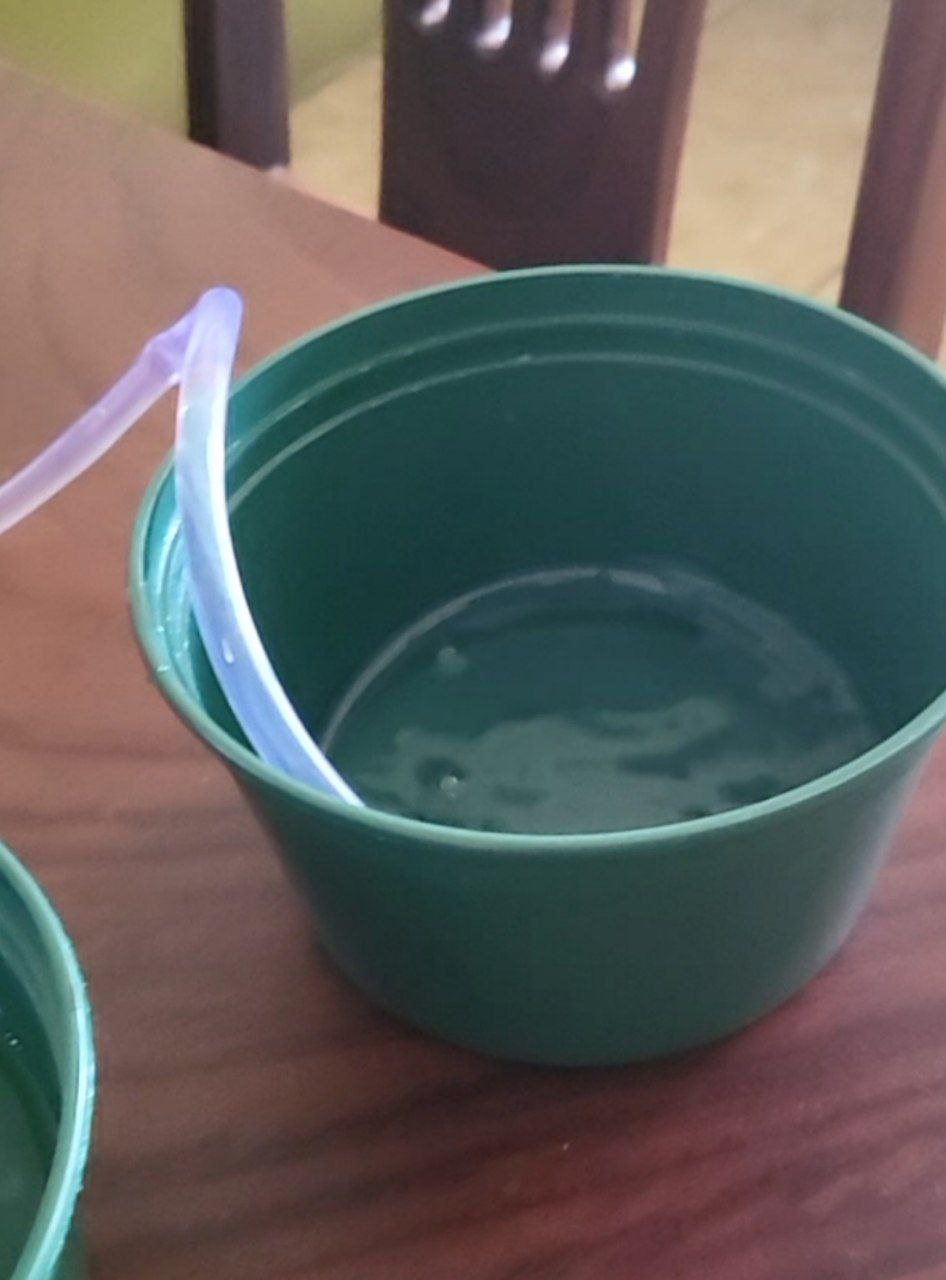
\includegraphics[width=80mm]{./Figuras/Desarrollo_Analisis/Llenado en progreso}
\caption{Imagen de taza de agua con el llenado en progreso.} 
\label{fig:analisis4}
\end{figure}
Mientras se esta realizando el llenado de la taza de agua, en terminal se obtiene la siguiente impresión:

\begin{figure}[H]
\centering
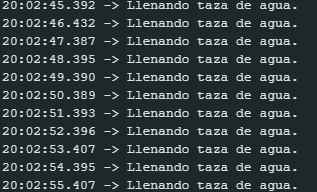
\includegraphics[width=80mm]{./Figuras/Desarrollo_Analisis/serial_llenando_agua}
\caption{Impresión con Serial monitor con llenado en progreso de taza de agua.} 
\label{fig:analisis5}
\end{figure}

A continuación una foto del \textit{dashboard} de Blynk con el llenado en progreso:

\begin{figure}[H]
\centering
\includegraphics[width=80mm]{./Figuras/Desarrollo_Analisis/Llenando agua}
\caption{\textit{Dashboard} con llenado en progreso de taza de agua.} 
\label{fig:analisis6}
\end{figure}

Al finalizar el llenado, se imprime lo siguiente en terminal:

\begin{figure}[H]
\centering
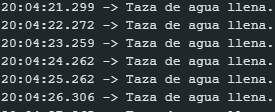
\includegraphics[width=80mm]{./Figuras/Desarrollo_Analisis/serial_agua_llena}
\caption{Impresión con Serial monitor con taza de agua llena.} 
\label{fig:analisis7}
\end{figure}
 
De este escenario, se observa un funcionamiento fluido y coherente entre los diferentes componentes del sistema. Al iniciar la acción desde Blynk, se verifica en el serial monitor que las impresiones de agua se realizan según lo esperado, confirmando que la bomba está operando correctamente. Además, en el \textit{dashboard} de Blynk se registra un progreso continuo y preciso en las mediciones de los niveles de agua, reflejando de manera efectiva el aumento en la cantidad de agua en la taza. Este escenario resalta la integración efectiva entre el control remoto mediante Blynk, la respuesta adecuada de los sensores y la visualización en tiempo real de los datos.

% CASO C llenando taza comida / Impresión en terminal X/ Foto del Dashboard X
\subsection{Caso C: Llenando taza de Comida}
A continuación se analiza el escenario en el se acciona el botón de llenar taza de comida

\begin{figure}[H]
\centering
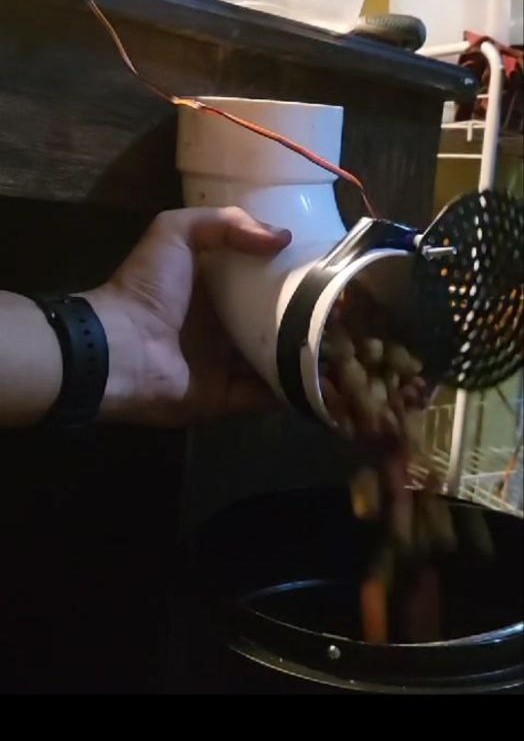
\includegraphics[width=80mm]{./Figuras/Desarrollo_Analisis/comida_progreso}
\caption{Imagen de Dispensador con llenado en progreso.} 
\label{fig:analisis8}
\end{figure}
Mientras se esta realizando el llenado de la taza de comida, en terminal se obtiene la siguiente impresión:

\begin{figure}[H]
\centering
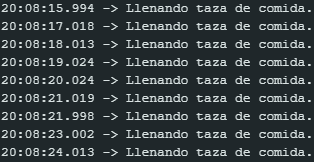
\includegraphics[width=80mm]{./Figuras/Desarrollo_Analisis/serial_llenando_comida}
\caption{Impresión con Serial monitor con llenado en progreso de taza de comida.} 
\label{fig:analisis9}
\end{figure}

A continuación una foto del \textit{dashboard} de Blynk con el llenado en progreso:

\begin{figure}[H]
\centering
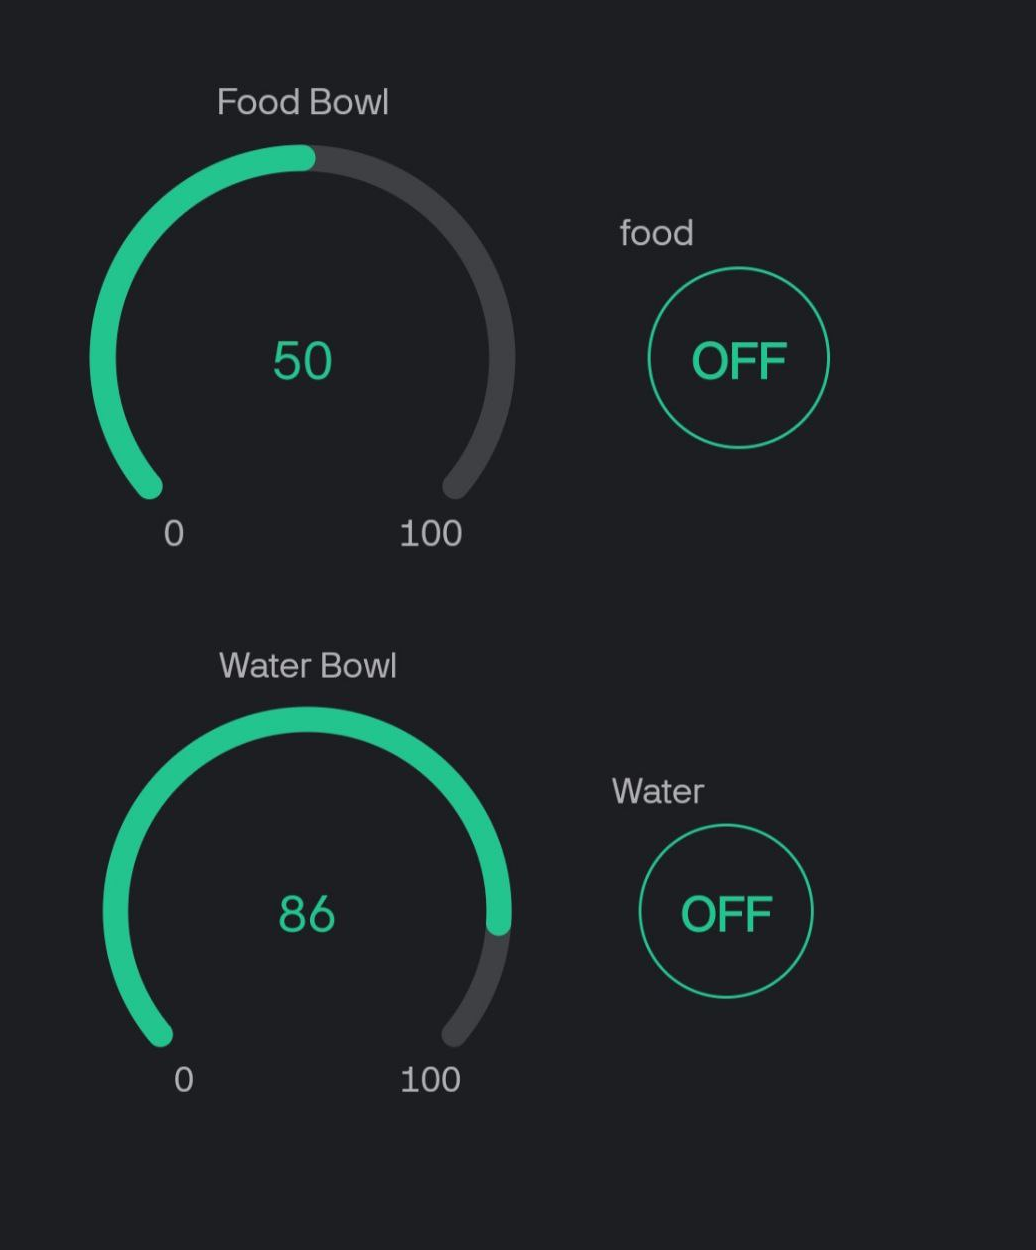
\includegraphics[width=80mm]{./Figuras/Desarrollo_Analisis/dash Llenando comida}
\caption{\textit{Dashboard} con llenado en progreso de taza de comida.} 
\label{fig:analisis10}
\end{figure}

Al finalizar el llenado, se imprime lo siguiente en terminal:

\begin{figure}[H]
\centering
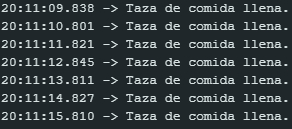
\includegraphics[width=80mm]{./Figuras/Desarrollo_Analisis/serial_comida_llena}
\caption{Impresión con Serial monitor con taza de comida llena.} 
\label{fig:analisis11}
\end{figure}
A continuación se muestra una imagen de ambas tazas llenas:

\begin{figure}[H]
\centering
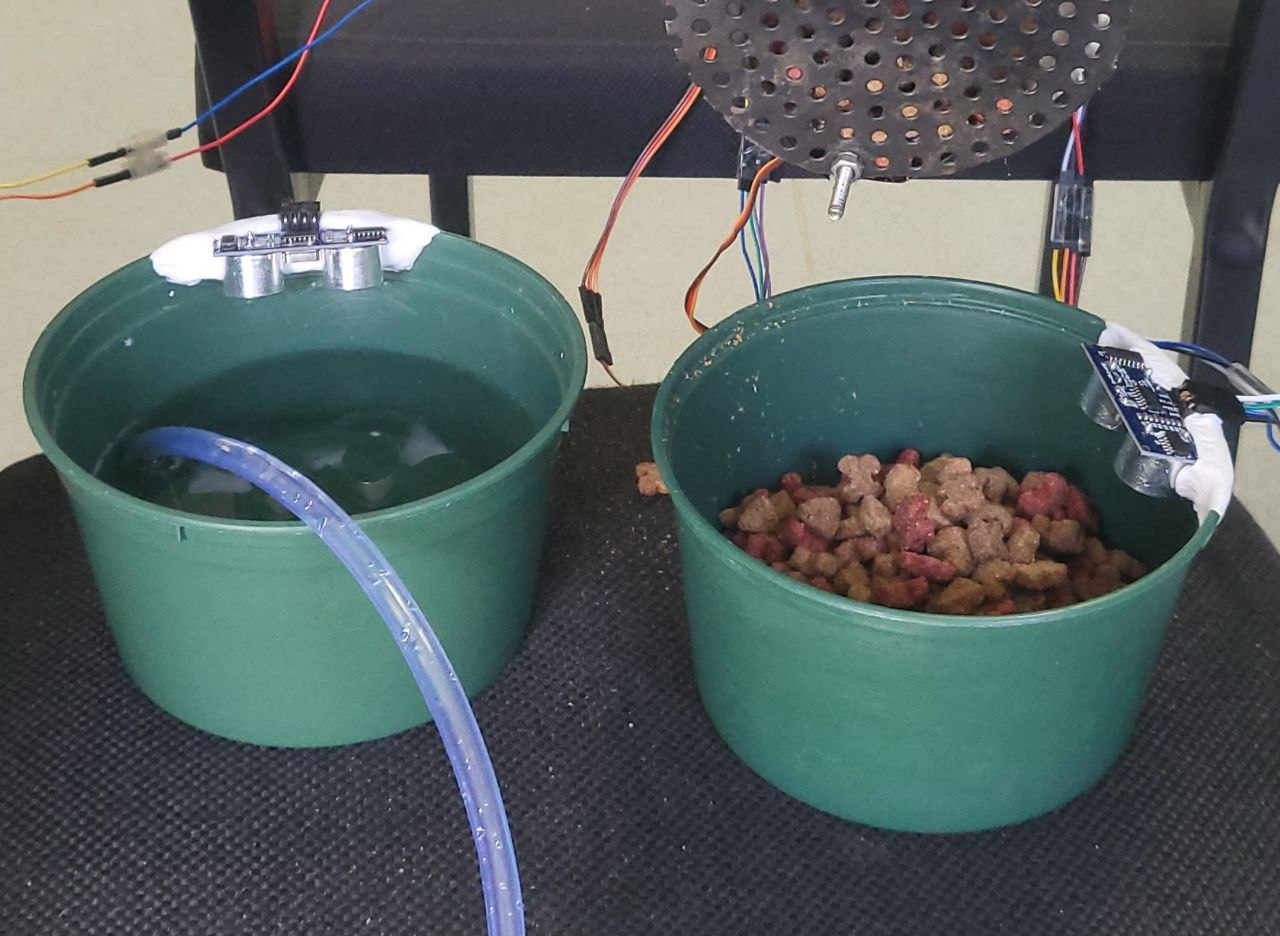
\includegraphics[width=80mm]{./Figuras/Desarrollo_Analisis/tazas_llenas}
\caption{Imagen del dispensador con tazas llenas.} 
\label{fig:analisis12}
\end{figure}

El \textit{dashboard} en este punto se muestra de la siguiente manera:

\begin{figure}[H]
\centering
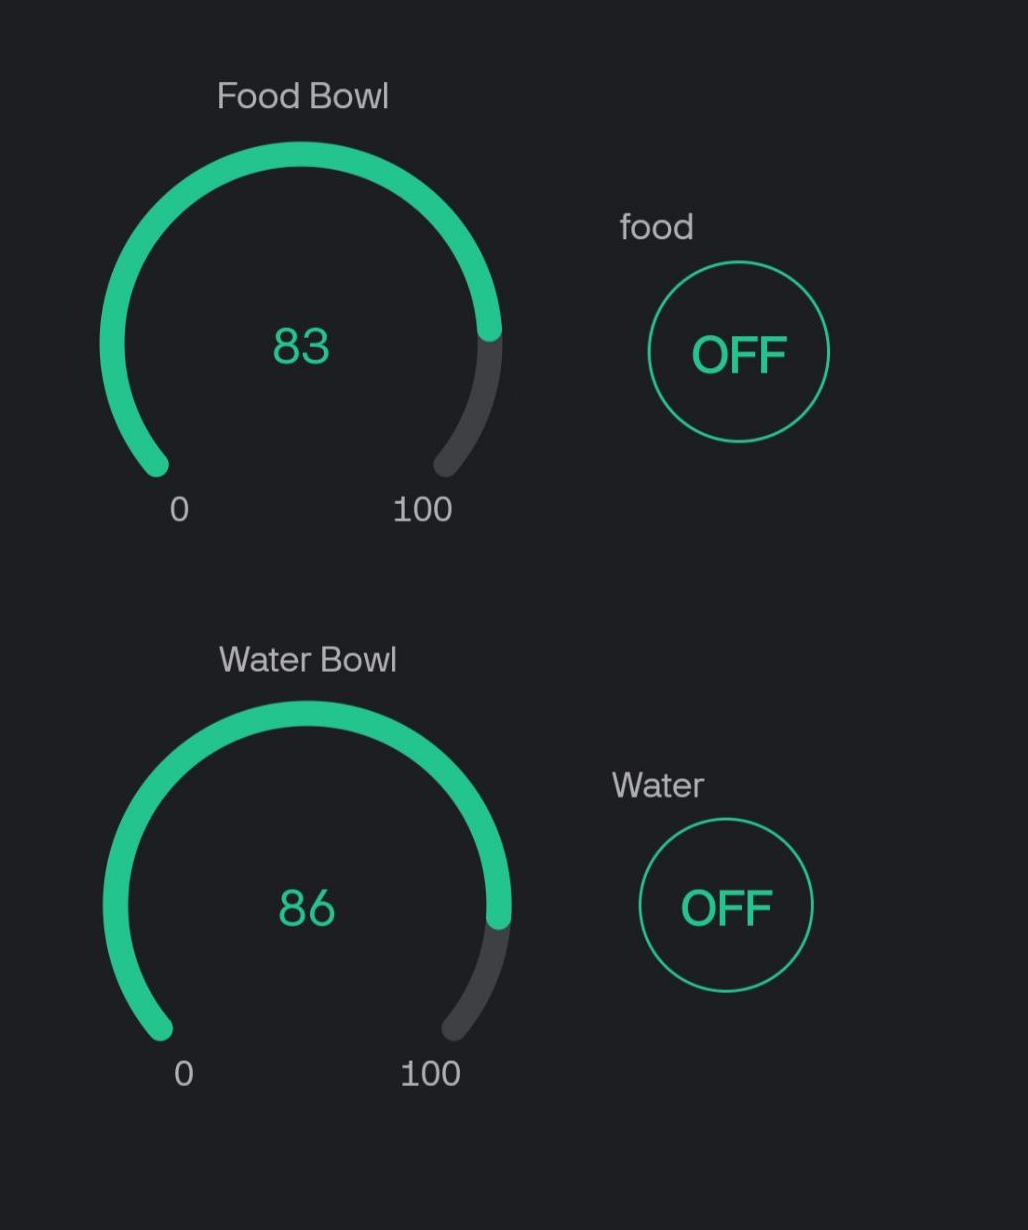
\includegraphics[width=80mm]{./Figuras/Desarrollo_Analisis/Ambos llenos}
\caption{\textit{Dashboard} con tazas llenas.} 
\label{fig:analisis13}
\end{figure}

De este ultimo escenario, se observa un desempeño robusto y coordinado del sistema. Al activar el servo motor a través de Blynk, el monitor serial proporciona retroalimentación en tiempo real con impresiones que indican el progreso del llenado, confirmando la operación adecuada del servo motor y la distribución de comida. El dashboard de Blynk refleja de manera precisa y progresiva el aumento en el nivel de comida en la taza, mostrando una sincronización efectiva entre la acción iniciada y la visualización de datos. 